\chapter{Assignment-Hamiltonian Equation of Motion}
\textbf{Assignment 01}
\begin{enumerate}
	\item A particle of inass $m$ moves inside a bowl under gravity. If the surface of the bowl is given by the equation $z=\frac{1}{2} a\left(x^{2}+y^{2}\right)$, where $a$ is a constant.\\
	(A) Write down Lagrangian of the system in cylindrical co-ordinate.\\
	(a) Identified the cyclic coordinate and law of conservation of momentum.\\
	(b) Write down hamiltonion of the system in cylindrical coordinate system.
	 \item A bike stuntman rides inside a well of frictionless surface given by $z=a\left(x^{2}+y^{2}\right)$, under the action of gravity acting in the negative $z$ direction i.e $\vec{g}=-g \hat{z}$. What speed should be maintain to be able to ride at a constant height $z_{0}$ without falling down?
	 \item A block of mass $M$ is suspended vertically from the cciting by a spring of spring constant $k$. A pendulum of mass $m$ is attached to the bottom of this block by a mass less rod of length $l$ (as shown in the attached figure). Assume that the block can move only vertically and that the motion of the pendulum takes place in a fixed vertical plane.\\
	 (a) Write down Lagrangian of the system in suitable generalized coordinate.\\
	 (b) write down Lagranges equation of motion.
	 \begin{figure}[H]
	 	\centering
	 	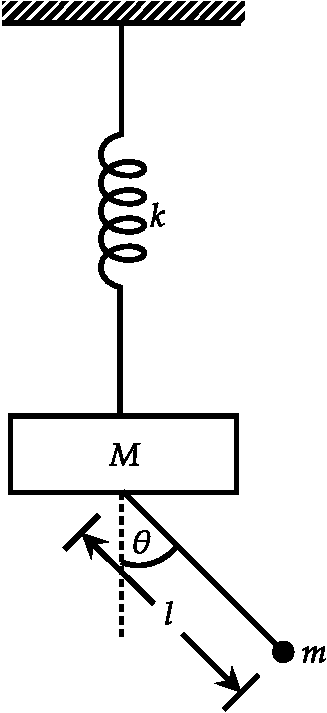
\includegraphics[height=5cm,width=2.5cm]{Assignment-HE-01}
	 \end{figure}
	 \item A particle of mass $m$ is attached to fixed point $O$ by a weightless inextensible string of length $a$. It is rotating under the gravity as shown in the figure.\\
	 (a) Write down The Lagrangian of the system in spherical co-ordinate.\\
	 (b) write down Hamiltonian of the system.
	  \begin{figure}[H]
	 	\centering
	 	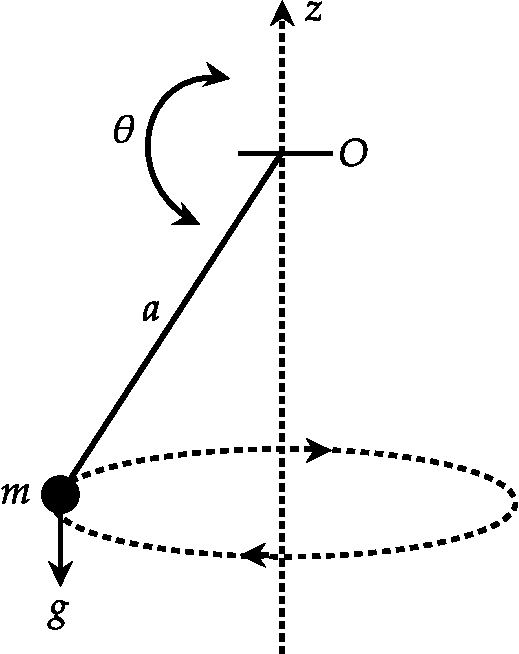
\includegraphics[height=4.5cm,width=3.5cm]{Assignment-HE-02}
	 \end{figure}
	 \item Particle of mass $m$ slides under the gravity without friction along the parabotic path
	 $y=a x^{2}$ axis shown in the figure. Here $a$ is a constant\\
	 (a) Write down Lagrangian of the system .\\
	 (b) Write down Lagranges equation of motion.\\
	 (c) write down Hamiltonian of the system.
	  \begin{figure}[H]
	 	\centering
	 	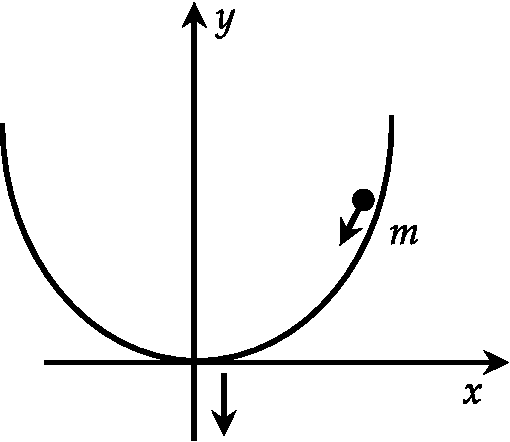
\includegraphics[height=3.5cm,width=4cm]{Assignment-HE-03}
	 \end{figure}
	 \item The Lagrangian of a particle of mass $m$ moving in one dimension is $L=\exp (\alpha t)\left[\frac{m \dot{x}^{2}}{2}-\frac{k x^{2}}{2}\right]$, where $\alpha$ and $k$ are positive constants.\\
	 (a) Find the Lagranges equation of motion of the particle.\\
	 (b) Write down Hamiltonian of the system.
	 \item A simple pendulum of mass $m_{2}$, with a mass $m_{1}$ at the point of support which can move on a horizontal line lying in the plane in which $m_{2}$ moves (Figure given)\\
	 (a) Write down Lagrangian of system.\\
	 (b) Which coordinate is cyclic co-ordinate.\\
	 (c) Find the generalized momentum.
	  \begin{figure}[H]
	 	\centering
	 	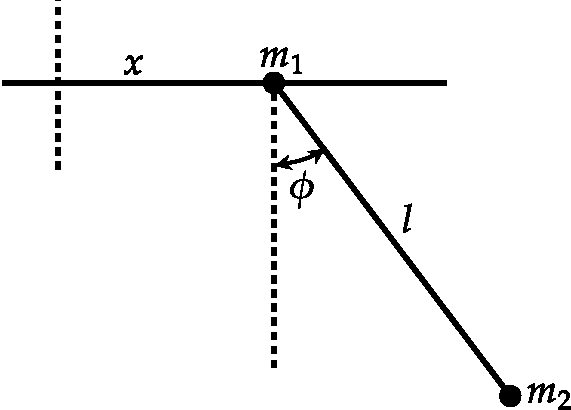
\includegraphics[height=4cm,width=5cm]{Assignment-HE-04}
	 \end{figure}
	 \item The point of support of a simple pendulum of length $b$. moves on a massless rim of a radius a rotating with constant angular velocity $\omega$.\\
	 (a) Obtain the expression for the Cartesian components of the velocity and acceleration and acceleration of the mass $m$.\\
	 (b) Write down expression of Lagrangian of a system in as function of $\omega$ and $\theta$\\
	 (c) Write down equation of motion of system.
	  \begin{figure}[H]
	 	\centering
	 	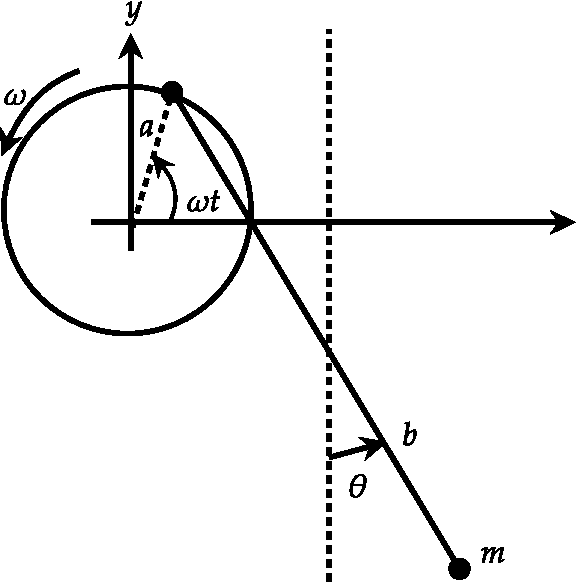
\includegraphics[height=5.5cm,width=5.5cm]{Assignment-HE-05}
	 \end{figure}
	 \item As shown in figure the particle of mass $m_{2}$ moves on a vertical axis and the whole system rotates about this axis with a constant angular velocity $\omega$.
	  \begin{tasks}(1)
	 	\task[\textbf{a.}] What is degree of freedom of system
	 	\task[\textbf{b.}] Write down Lagrangian of the system in spherical polar co-ordinate.
	 	\task[\textbf{c.}]Write down Lagranges equation of the system.
	 	\task[\textbf{d.}] Write down Hamiltonian of the system.
	 \end{tasks}
  \begin{figure}[H]
 	\centering
 	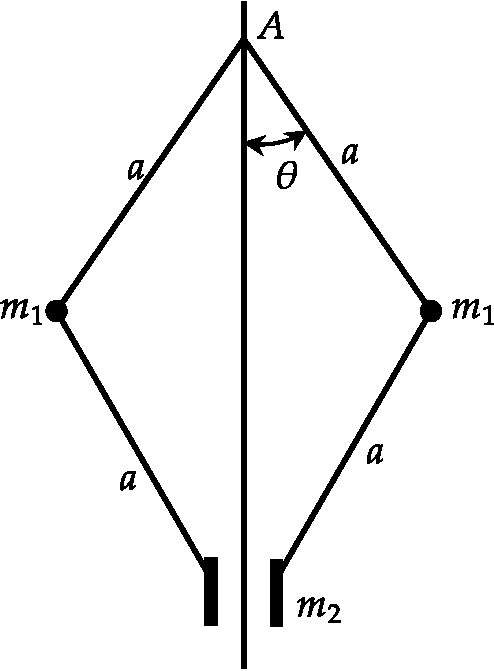
\includegraphics[height=6cm,width=3.6cm]{Assignment-HE-06}
 \end{figure}
	 \item A bead of mass $m$ can slide without friction along a mass less rod kept at $45^{\circ}$ with the vertical as shown in the figure. The rod is rotating about the vertical axis with a constant angular speed $\omega$. At any instant $r$ is the distance of the bead from the origin.\\
	 (a) Find the Lagrangian of the system\\
	 (b) Find the momentum conjugate to $r$.
	  \begin{figure}[H]
	 	\centering
	 	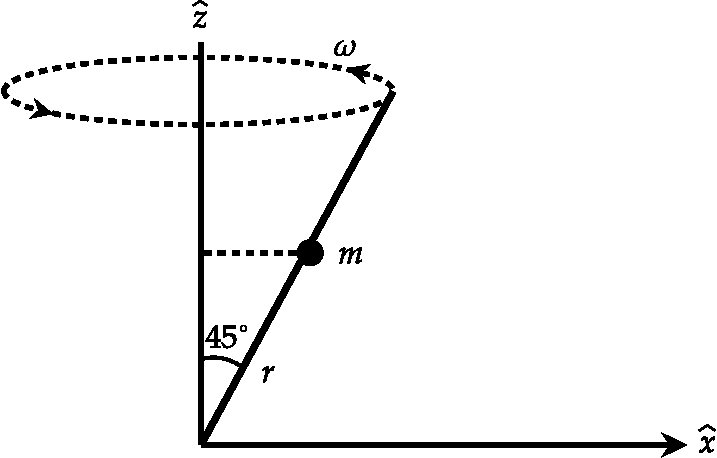
\includegraphics[height=4.5cm,width=6.5cm]{Assignment-HE-07}
	 \end{figure}
	 \item A bead slides along a smooth wire bent in the shape of a parabola $z=c r^{2}$ (figure). The bead rotates in a circle of radius $R$ when the wire is rotating about its vertical symmetry axis with angular velocity $\omega$. Find the value of $c$.
	  \begin{figure}[H]
	 	\centering
	 	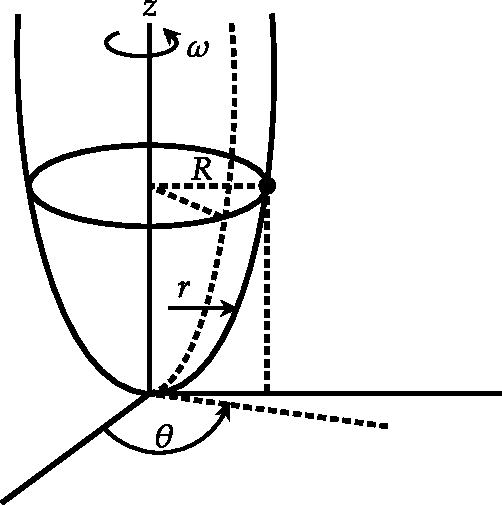
\includegraphics[height=6cm,width=5.2cm]{Assignment-HE-08}
	 \end{figure}
\end{enumerate}
\textbf{Assignment 02}
\begin{enumerate}
	\item A system is governed by the Hamiltonian
	$$
	I=\frac{1}{2}\left(p_{x}-a y\right)^{2}+\frac{1}{2}\left(p_{y}-b x\right)^{2}
	$$
	where $a$ and $b$ are constants and $p, p$, are momenta conjugate to $x$ and $y$ respectively. For what values of $a$ and $b$ will the quantities $\left(p_{x}-3 y\right)$ and $\left(p_{y}+2 x\right)$ be conserved.
	\item A particle of mass $m$ and coordinate $q$ has the Lagrangian $L=\frac{1}{2} m \dot{q}^{2}-\frac{\lambda}{2}-\dot{q}^{2}$ where $\lambda$ is a constant. Find the Hamiltonian of the system.
	\item The coordinates and momenta $x_{i}, \quad p_{i}(i=1,2,3)$ of a particle satisfy the canonical Poisson bracket relations $\left\{x_{i}, p_{j}\right\}=\delta_{i j}$. If $C_{1}=x_{2} p_{3}+x_{3} p_{2}, C_{2}=x_{1} p_{2}-x_{2} p_{1}$ and $C_{3}=x_{1} p_{3}+x_{3} p_{1} .$ Then\\
	(a) Find the value of $\left\{C_{1}, C_{2}\right\}$\\
	(b) Find the relation between $C_{1}, C_{2}$ and $C_{3}$.
	\item If Hamiltonian of the Harmonic oscillator is given by $H=\frac{p^{2}}{2 m}+\frac{1}{2} m \omega^{2} x^{2}$, the quantity defined $u(x, p, t)=\ln (p+i m \omega x)-i \omega t$ then check whether $u$ is conserve during the motion.
	\item The Hamiltonian of a particle of unit mass moving in the $x y$-plane is given to be: $H=x p_{x}-y p_{y}-\frac{1}{2} x^{2}+\frac{1}{2} y^{2}$ in suitable units. The initial values are given to be $(x(0), y(0))=(1,1)$ and $\left(p_{x}(0), p_{y}(0)\right)=\left(\frac{1}{2}, \frac{1}{2}\right)$.\\
	(a) Discuss equation of motion\\
	(b) Plot the curves traced out by the particles in the $x y$-plane and the $p_{x} p_{y}-$ plane.
	\item A mechanical system is described by the Hamiltonian $H(q, p)=\frac{p^{2}}{2 m}-\frac{1}{2} m \omega^{2} q^{2} .$ As a result of the canonical transtormation generated by $F(q, Q)=-\frac{Q}{q}$, the Hamiltonian in the new coordinate $Q$ and momentum $P$.
	\item The Hamiltonian of the system is given by $H=\frac{p_{x}^{2}}{2 m}+\frac{p_{y}^{2}}{2 m}+\frac{m \omega^{2}\left(x^{2}+y^{2}\right)}{2}$. Check whether the following quantities are conserve during the motion or not.\\
	(a) $S_{1}=\frac{1}{2}\left(x p_{y}-y p_{x}\right)$\\
	(b) $S_{2}=\frac{1}{2 m \omega}\left(p_{x} p_{1}+m^{2} \omega^{2} x y\right)$\\
	(c) $S_{3}=\frac{1}{4 m \omega}\left[p_{s}^{2}-p_{3}^{2}+m^{2} \omega^{2}\left(y^{2}-x^{2}\right)\right]$\\
	\item The transformation equations between two sets of coordinate are
	$$
	\begin{aligned}
	&Q=\log \left(1+q^{1 / 2} \cos p\right) \\
	&P=2\left(1+q^{1 / 2} \cos p\right) q^{1 / 2} \sin p
	\end{aligned}
	$$\
	(a) Show that $Q, P$ are canonical transform to $q, p$.\\
	(b) Show that the function that generates this transformation is $F_{3}=-\left(e^{Q}-1\right)^{2} \tan p$
	\item Prove that the transformation is canonical.\\
	(i) $Q_{1}=q_{1}, P_{1}=p_{1}-2 p_{2}$,\\
	(ii) $Q_{2}=p_{2}, P_{2}=-2 q_{1}-q_{2}$
	\item  The Hamiltonian of harmonic oscillator is given by $H=\frac{1}{2 m}\left(p^{2}+m^{2} \omega^{2} q^{2}\right)$\\
 	A. \begin{tasks}(1)
		\task[\textbf{a.}]Write down equation of motion
		\task[\textbf{b.}]Plot phase space for given energy $E$
		\task[\textbf{c.}] Plot $q$ vs $t$ with initial condition $t=0, q=q_{0}$ and $\dot{q}-0$ at $t=0$
		\task[\textbf{d.}] Plot $p$ vs $t$
	\end{tasks}
	B.	 \begin{tasks}(1)
		\task[\textbf{a.}] (a) If a generating function is defined as $F_{1}=\frac{m \omega q^{2}}{2} \cot Q$ then find canonical transformation.\\
		From the use of canonical transformation $H=\frac{1}{2 m}\left(p^{2}+m^{2} \omega^{2} q^{2}\right)$
		\task[\textbf{b.}]Find new Hamiltonian $K(Q, P, t)$
		\task[\textbf{c.}]Plot $Q$ vs $t$
		\task[\textbf{d.}]Plot $P$ vs $t$
		\task[\textbf{e.}]Plot phase space between $P$ and $Q$
	\end{tasks}
\item If generating function is given by $F(q, P)=q^{2} P$ and Hamiltonian of the system is given by $H(q, p)=\frac{p^{2}}{2 \alpha q^{2}}+\frac{\beta q^{4}}{4}$ where $\alpha$ and $\beta$ are constants, then find the equation of motion in term of $Q, P$.
\item If Lagrangian of the system is given by $L=\frac{1}{2} m \dot{x}^{2}+m\left(\dot{y}^{2}+\dot{z}^{2}\right)-\frac{1}{2} k x^{2}-\frac{1}{2} k(y+z)^{2}$
 \begin{tasks}(2)
	\task[\textbf{a.}]Write down Hamiltonian of system.
	\task[\textbf{b.}]If $L_{z}=x p_{y}-y p_{x}$, find $\frac{d L_{z}}{d t}$
	\task[\textbf{c.}]If $L_{x}=y p_{z}-z p_{y}$, find $\frac{d L_{x}}{d t}$
	\task[\textbf{d.}] If $L_{y}=z p_{x}-x p_{z}$, find $\frac{d L_{y}}{d t}$
	\task[\textbf{e.}]Find $\frac{d p_{x}}{d t}$ and $\frac{d p_{y}}{d t}$
\end{tasks}
	
	
	
	
	
	
	
	
	
	
	
	
	
	
	
	
	
	
	
\end{enumerate}

